\documentclass[
    table,
    12pt,
    oneside,
    a4paper,
    italian
]{book}

\PassOptionsToPackage{dvipsnames}{xcolor} % colori PDF/A

\usepackage{colorprofiles}
% PDF/A
% validate in https://www.pdf-online.com/osa/validate.aspx
\usepackage[a-1a,mathxmp]{pdfx}[2018/12/22]
\usepackage[T1]{fontenc}
\usepackage[utf8]{inputenc}
\usepackage[italian]{babel}
\usepackage{bookmark}
\usepackage{caption}
\usepackage{comment}
\usepackage{chngpage, calc} % centra il frontespizio
\usepackage{emptypage} % pagine vuote senza testatina e piede di pagina
\usepackage{epigraph} % per epigrafi
\usepackage{indentfirst} % rientra il primo paragrafo di ogni sezione
\usepackage{graphicx} % immagini
\usepackage[pdfa]{hyperref} % collegamenti ipertestuali
\usepackage{mparhack,relsize}  % finezze tipografiche
\usepackage{nameref} % visualizza nome dei riferimenti
\usepackage[font=small]{quoting} % citazioni
\usepackage{subfig} % sottofigure, sottotabelle
\usepackage[italian]{varioref} % riferimenti completi della pagina
\usepackage{longtable} % tabelle su più pagine
\usepackage[toc, acronym, automake]{glossaries}
\usepackage[backend=biber, style=verbose-ibid, hyperref, backref]{biblatex}
\usepackage{lmodern}
\usepackage[top=2.75cm, bottom=2.75cm, right=3cm, left=3.75cm]{geometry} % 1in+17pt+0.6cm
\usepackage{fancyhdr}
\usepackage{lipsum}
\usepackage{setspace}
\usepackage{titlesec}
\usepackage[cachedir=minted-caches]{minted} % https://it.overleaf.com/learn/latex/Code_Highlighting_with_minted
\usepackage{xcolor}
\usepackage{csquotes} % gestisce automaticamente i caratteri (")
\usepackage{etoolbox}
\usepackage[bottom]{footmisc}
\usepackage{zref-totpages}
% Load variables
\newcommand{\myUni}{Università degli Studi di Padova}
\newcommand{\myDepartment}{Dipartimento di Matematica ``Tullio Levi-Civita''}
\newcommand{\myFaculty}{Corso di Laurea in Informatica}
\newcommand{\myTitle}{Un sistema Honeypot per l'analisi di attacchi informatici in ambiente controllato}
\newcommand{\myDegree}{Tesi di Laurea Triennale}
\newcommand{\profTitle}{Prof.}
\newcommand{\myProf}{Vardanega Tullio}
\newcommand{\graduateTitle}{Laureando}
\newcommand{\myName}{Marko Peric}
\newcommand{\myStudentID}{2011067}
\newcommand{\myAA}{2024-2025}
\newcommand{\myLocation}{Padova}
\newcommand{\myTime}{Agosto 2025}
% Acronyms
\newacronym{tsa}{TSA}{Termine solo acronimo}

% Glossary

\newglossaryentry{TermineSenzaAcronimo}{
    name={Nome del termine},
    sort=termine senza acronimo,
    description={Descrizione}
}
\PassOptionsToPackage{dvipsnames}{xcolor} % colori PDF/A

\usepackage{colorprofiles}
% PDF/A
% validate in https://www.pdf-online.com/osa/validate.aspx
\usepackage[a-1a,mathxmp]{pdfx}[2018/12/22]
\usepackage[T1]{fontenc}
\usepackage[utf8]{inputenc}
\usepackage[italian]{babel}
\usepackage{bookmark}
\usepackage{caption}
\usepackage{comment}
\usepackage{chngpage, calc} % centra il frontespizio
\usepackage{emptypage} % pagine vuote senza testatina e piede di pagina
\usepackage{epigraph} % per epigrafi
\usepackage{indentfirst} % rientra il primo paragrafo di ogni sezione
\usepackage{graphicx} % immagini
\usepackage[pdfa]{hyperref} % collegamenti ipertestuali
\usepackage{mparhack,relsize}  % finezze tipografiche
\usepackage{nameref} % visualizza nome dei riferimenti
\usepackage[font=small]{quoting} % citazioni
\usepackage{subfig} % sottofigure, sottotabelle
\usepackage[italian]{varioref} % riferimenti completi della pagina
\usepackage{longtable} % tabelle su più pagine
\usepackage[toc, acronym, automake]{glossaries}
\usepackage[backend=biber, style=verbose-ibid, hyperref, backref]{biblatex}
\usepackage{lmodern}
\usepackage[top=2.75cm, bottom=2.75cm, right=3cm, left=3.75cm]{geometry} % 1in+17pt+0.6cm
\usepackage{fancyhdr}
\usepackage{lipsum}
\usepackage{setspace}
\usepackage{titlesec}
\usepackage[cachedir=minted-caches]{minted} % https://it.overleaf.com/learn/latex/Code_Highlighting_with_minted
\usepackage{xcolor}
\usepackage{csquotes} % gestisce automaticamente i caratteri (")
\usepackage{etoolbox}
\usepackage[bottom]{footmisc}
\usepackage{zref-totpages}

% Define custom colors
\definecolor{hyperColor}{HTML}{0B3EE3}
\definecolor{tableGray}{HTML}{F5F5F7}
\definecolor{veryPeri}{HTML}{6667ab}

% Set line height
\linespread{1.5}

% Custom hyphenation rules
\hyphenation {
    data-base
    al-go-rithms
    soft-ware
}

% Images path
\graphicspath{{img/}}

% Force page color, as some editors set a grayish color as default
\pagecolor{white}

% Better spacing for footnotes
\setlength{\skip\footins}{5mm}
\setlength{\footnotesep}{5mm}

\setlength{\headheight}{14.5pt}
\addtolength{\topmargin}{-2.45pt}

% Add a subscript G to a glossary entry
\newcommand{\glox}{\textsubscript{\textbf{\textit{G}}}}

% Improvements the paragraph command
\titleformat{\paragraph}
{\normalfont\normalsize\bfseries}{\theparagraph}{1em}{}
\titlespacing*{\paragraph}
{0pt}{3.25ex plus 1ex minus .2ex}{1.5ex plus .2ex}

% Define use case environment
\newcounter{usecasecounter} % define a counter
\setcounter{usecasecounter}{0} % set the counter to some initial value
% Parameters
% #1: ID
% #2: Nome
\newenvironment{usecase}[2]{
    \renewcommand{\theusecasecounter}{\usecasename #1}  % this is where the display of the counter is overwritten/modified
    \refstepcounter{usecasecounter} % increment counter
    \vspace{2em}
    \par \noindent % start new paragraph
    {\normalsize \textbf{\usecasename #1: #2}} % display the title before the content of the environment is displayed
    \vspace{.5em}
}{
    \medskip
}
\newcommand{\usecasename}{UC}
\newcommand{\usecaseactors}[1]{\textbf{\\Attori Principali:} #1}
\newcommand{\usecasepre}[1]{\textbf{\\Precondizioni:} #1}
\newcommand{\usecasedesc}[1]{\textbf{\\Descrizione:} #1}
\newcommand{\usecasepost}[1]{\textbf{\\Postcondizioni:} #1}
\newcommand{\usecasealt}[1]{\textbf{\\Scenario Alternativo:} #1}

% Define risks environment
\newcounter{riskcounter} % define a counter
\setcounter{riskcounter}{0} % set the counter to some initial value
% Parameters
% #1: Title
\newenvironment{risk}[1]{
    \refstepcounter{riskcounter} % increment counter
    \par \noindent % start new paragraph
    \textbf{\arabic{riskcounter}. #1} % display the title before the content of the environment is displayed
}{
    \par\medskip
}
\newcommand{\riskname}{Rischio}
\newcommand{\riskdescription}[1]{\textbf{\\Descrizione:} #1.}
\newcommand{\risksolution}[1]{\textbf{\\Soluzione:} #1.}

% Apply fancy styling to pages
\pagestyle{fancy}
\fancyhf{}
\fancyhead[L]{\leftmark} % Places Chapter N. Chatper title on the top left
\fancyfoot[C]{\thepage} % Page number in the center of the footer

% Adds a blank page while increasing the page number
\newcommand\blankpage{ 
\clearpage
    \begingroup
    \null
    \thispagestyle{empty}
    \hypersetup{pageanchor=false}
    \clearpage
\endgroup
}

% Adds a blank page while increasing the page number
\newcommand\blankpagewithnumber{ 
  \clearpage
  \thispagestyle{plain} % Use plain page style to keep the page number
  \null
  \clearpage
}

% Increase page numbering
\newcommand\increasepagenumbering{
    \addtocounter{page}{+1}
}

% Make glossaries and bibliography
\makeglossaries
% Redefine the format for the glossary entries to be italic
\renewcommand*{\glstextformat}[1]{\textit{#1}\glox}
%\glsaddall

\bibliography{references/bibliography}
\defbibheading{bibliography} {
    \cleardoublepage
    \phantomsection
    \addcontentsline{toc}{chapter}{\bibname}
    \chapter*{\bibname\markboth{\bibname}{\bibname}}
}

% Code blocks handling w/ table of codes
\makeatletter
\ifdefined\NR@chapter
  \expandafter\@firstoftwo
\else
  \expandafter\@secondoftwo
\fi{\patchcmd\NR@chapter}{\patchcmd\@chapter}
  {\addtocontents{lot}{\protect\addvspace{10\p@}}}
  {\addtocontents{lot}{\protect\addvspace{10\p@}}%
   \addtocontents{lol}{\protect\addvspace{10\p@}}}
  {}{}
\makeatother

\renewcommand\listingscaption{Codice}
\renewcommand\listoflistingscaption{Elenco dei codici sorgenti}
\counterwithin*{listing}{chapter}
\renewcommand\thelisting{\thechapter.\arabic{listing}}

% Set up hyperlinks
\hypersetup{
    colorlinks=true,
    linktocpage=true,
    pdfstartpage=1,
    pdfstartview=,
    breaklinks=true,
    pdfpagemode=UseNone,
    pageanchor=true,
    pdfpagemode=UseOutlines,
    plainpages=false,
    bookmarksnumbered,
    bookmarksopen=true,
    bookmarksopenlevel=1,
    hypertexnames=true,
    pdfhighlight=/O,
    allcolors = hyperColor
}

% Set up captions
\captionsetup{
    tableposition=top,
    figureposition=bottom,
    font=small,
    format=hang,
    labelfont=bf
}

% When draft mode is on, the hyperlinks are removed. Useful when printing the document. To enable/disable, uncomment/comment the command
% \hypersetup{draft}

% prevents cleaning up the cache at the end of the run (needed to keep the unused caches, generated by other editions)
% \makeatletter
% \renewcommand*{\minted@cleancache}{}
% \makeatother

% Break lines in code blocks whe using inputminted
\setminted{breaklines}

\date{}

\hypersetup{pdfstartview=}
\begin{document}
    \frontmatter
    \begin{titlepage}
    \begin{center}
        \begin{Large}
            \textbf{\myUni}\\
        \end{Large}

        \vspace{5pt}

        \begin{large}
            \textsc{\myDepartment}\\
        \end{large}

        \vspace{5pt}

        \begin{large}
            \textsc{\myFaculty}\\
        \end{large}

        \vspace{25pt}
        
        \begin{figure}[htbp]
            \centering
            
\includegraphics[alt={Emblema dell'Università degli Studi di Padova}, height=6cm]{img/logo_unipd.jpeg}
        \end{figure}

        
        \begin{Large}
            \textbf{\myTitle}\\
        \end{Large}

        \vspace{5pt}

        \begin{large}
            \textit{\myDegree}\\
        \end{large}

        \vspace{50pt}
        
        \begin{normalsize}
            \begin{flushleft}
                \textit{Relatore}\\
                \profTitle\ \myProf
            \end{flushleft}

            \vspace{-48pt}
            
            \begin{flushright}
                \textit{\graduateTitle}\\
                \myName\\
                Matricola \myStudentID
            \end{flushright}
        \end{normalsize}

        \vspace*{\fill}
        
        \line(1, 0){338} \\
        \begin{normalsize}
            \textsc{Anno Accademico \myAA}
        \end{normalsize}
    \end{center}
\end{titlepage}

    \increasepagenumbering % increase the page numbrering by 1, in order to cout the frontispiece
    \clearpage
\phantomsection
\thispagestyle{empty}
\hfill
\vfill

{\small\noindent\textcopyright\ \myName, \myTime. Tutti i diritti riservati. \myDegree: ``\textit{\myTitle}'', \myUni, \myDepartment, \myFaculty.}
    \cleardoublepage
\phantomsection
\pdfbookmark{Ringraziamenti}{Ringraziamenti}

\begin{flushright}{
    \slshape
    ``Colui il quale ha inseguito e sconfitto i demoni Sem, che ora vagano per il mondo, domandandosi: «ma nü, chi sëm?»''} \\
    \medskip
    --- Il grande Pdor, figlio di Kmer, della tribù di Ishtar, della terra desolata dei Kfnir, uno degli ultimi sette saggi: Pfulur, Galér, Astaparigna, Sùsar, Param, Fusus e Tarìm.
\end{flushright}

\begingroup
\let\clearpage\relax
\let\cleardoublepage\relax
\let\cleardoublepage\relax

\chapter*{Ringraziamenti}

\noindent Desidero esprimere la mia gratitudine al professor \myProf, mio relatore, per l'aiuto e il sostegno che mi ha dato durante la stesura dell'elaborato.

\vspace{0.35cm}

\noindent Vorrei anche ringraziare, con affetto, i miei genitori per il loro sostegno, il grande aiuto e la loro presenza in ogni momento durante gli anni di studio.

\vspace{0.35cm}

\noindent Desidero poi ringraziare i miei amici per i bellissimi anni trascorsi insieme e le mille avventure vissute.

\vspace{0.75cm}

\noindent{\myLocation, \myTime}
\hfill \textit{\myName}

\endgroup

    \cleardoublepage
\phantomsection
\pdfbookmark{Compendio}{Compendio}
\begingroup
\let\clearpage\relax
\let\cleardoublepage\relax
\chapter*{Sommario}
Il presente elaborato descrive il lavoro svolto durante il periodo di \textit{stage}, della durata di circa
320 ore, dal laureando Marko Peric presso l'azienda Eurosystem S.p.A. dal 18/06/2024 al
13/08/2025.
L'elaborato illustra i processi, le metodologie e gli strumenti impiegati nella progettazione e nello sviluppo di un sistema \textit{honeypot} finalizzato al monitoraggio e alla rilevazione di attività malevole in rete. Il sistema si basa sull'installazione di servizi volutamente vulnerabili su un server Linux Debian, con lo scopo di attirare potenziali attaccanti e analizzarne i comportamenti. I \textit{log} generati dai servizi vengono successivamente raccolti, elaborati e trasferiti in InfluxDB per la loro conservazione, e resi disponibili tramite Grafana per consentire un'analisi e una visualizzazione efficace delle informazioni tramite \textit{dashboard}.
\section*{Struttura dell'elaborato}
In questa sezione viene presentata la struttura dell'elaborato, illustrando brevemente il contenuto di ciascun capitolo:
\begin{description}
    \item[{\hyperref[chap:]{Il primo capitolo}}] approfondisce il contesto aziendale in cui si è svolto lo \textit{stage}, fornendo una panoramica completa dell'azienda, dei suoi prodotti e servizi nel settore della \textit{cybersecurity}, degli strumenti tecnologici utilizzati e dell'organizzazione del \textit{team} di sicurezza informatica, analizzando inoltre l'approccio dell'azienda verso l'innovazione tecnologica;

    \item[{\hyperref[chap:]{Il secondo capitolo}}] identifica e analizza il problema alla base del progetto, definendo gli obiettivi specifici dello sviluppo del sistema \textit{honeypot}, i vincoli operativi e tecnici che hanno influenzato il lavoro, le prospettive di sviluppo futuro e le motivazioni personali che hanno guidato la scelta di questo percorso di \textit{stage};

    \item[{\hyperref[chap:]{Il terzo capitolo}}] documenta l'intero processo di sviluppo del sistema \textit{honeypot}, dall'analisi dei requisiti e dei casi d'uso alla progettazione dell'architettura, dalla fase di codifica alle attività di verifica e validazione, presentando il prodotto finale e valutando il grado di conformità rispetto ai requisiti iniziali;
    
    \item[{\hyperref[chap:]{Il quarto capitolo}}] presenta una valutazione retrospettiva dell'esperienza formativa, analizzando il raggiungimento degli obiettivi prefissati, le conoscenze tecniche acquisite nel campo della sicurezza informatica e le competenze professionali sviluppate durante il periodo di tirocinio presso l'azienda.
\end{description}
\section*{Criteri tipografici adottati}
Riguardo la stesura del testo, relativamente al elaborato sono state adottate le seguenti convenzioni tipografiche:
\begin{itemize}
	\item gli acronimi e le abbreviazioni sono raccolti in un'apposita sezione dedicata, denominata \hyperref[acronimi]{Elenco degli acronimi} e sono segnati con la seguente nomenclatura \gls{es};
    \item i termini ambigui o di uso non comune, invece, sono definiti all'interno del \hyperref[glossario]{Glossario} e sono segnati con la seguente nomenclatura \gls{esempio};
	\item i termini in lingua straniera o facenti parti del gergo tecnico sono evidenziati con il carattere \textit{corsivo}.
\end{itemize}
\endgroup
\vfill

    \cleardoublepage
\pdfbookmark{\contentsname}{tableofcontents}
\setcounter{secnumdepth}{5}
\setcounter{tocdepth}{5}     

\tableofcontents
\clearpage

\begingroup
    \let\clearpage\relax
    \let\cleardoublepage\relax
    \let\cleardoublepage\relax

    % Figures list
    \phantomsection
    \pdfbookmark{\listfigurename}{lof}
    \listoffigures
    \vspace*{8ex}

    % Tables list
    \phantomsection
    \pdfbookmark{\listtablename}{lot}
    \listoftables
\endgroup

\begingroup
    % Code list
    \phantomsection
    \pdfbookmark{\listoflistingscaption}{lol}
    \listoflistings
\endgroup

\cleardoublepage
    \printglossary[type=\acronymtype, title=Acronimi e abbreviazioni, toctitle=Acronimi e abbreviazioni]
    \printglossary[type=main, title=Glossario, toctitle=Glossario]
    \blankpage % example of a blank page that also increases the page couter by 1

    \mainmatter
    \chapter{Introduzione}
\label{chap:introduzione}
\section{L'azienda}
Paragrafo che conterrà la descrizione dell'azienda scelta in cui è stato effettuato lo stage (Eurosystem S.p.A.).
% Eurosystem S.p.A. è un'azienda informatica che si occupa di consulenza, prodotti e servizi IT. Dal 2022, fa parte del Gruppo internazionale Smart4Engineering, leader europeo nella trasformazione digitale.
% Presenta 8 sedi in Nord e Centro Italia (Treviso, Bergamo, Bologna, Udine, Ferrara, Modena, Milano, Firenze) supportando oltre 1300 clienti di piccola e media impresa.
% Ad oggi offre soluzioni nei settori delle Business Applications e Industria 4.0, delle Immersive Technologies, della Cyber Security e delle Tech Solutions \& Services.\\
% Il logo dell'azienda è riportato in figura \ref{fig:logo_eurosystem}
\begin{figure}[H]
    \centering
    
\includegraphics[alt={Testo alternativo dell'immagine}, width=0.4\columnwidth]{img/logo_azienda.png}
    \caption{Logo di Eurosystem S.p.A.}
    \label{fig:logo_eurosystem}
\end{figure} 

\section{L'idea}
Paragrafo che conterrà la descrizione dell'idea di stage proposta dall'azienda e come questa sia stata implementata in maniera sintetica.
%Lo stage proposto consiste nell'implementare un sistema honeypot per la rilevazione delle minacce informatiche. Il sistema sarà progettato per simulare vulnerabilità e attirare attacchi, consentendo così di analizzare le tecniche utilizzate dagli aggressori e migliorare le difese informatiche.

\section{Organizzazione del testo}
In questa sezione viene presentata la struttura del documento, illustrando brevemente il contenuto di ciascun capitolo. Inoltre, vengono descritte le principali convenzioni adottate per la stesura, tra cui le modalità di scrittura degli acronimi, dei termini presenti nel glossario e dei termini in lingua straniera o tecnico-specialistica.
% \begin{description}
%     \item[{\hyperref[chap:processi-metodologie]{Il secondo capitolo}}] descrive ...
    
%     \item[{\hyperref[chap:descrizione-stage]{Il terzo capitolo}}] approfondisce ...
    
%     \item[{\hyperref[chap:analisi-requisiti]{Il quarto capitolo}}] approfondisce ...
    
%     \item[{\hyperref[chap:progettazione-codifica]{Il quinto capitolo}}] approfondisce ...
    
%     \item[{\hyperref[chap:verifica-validazione]{Il sesto capitolo}}] approfondisce ...
    
%     \item[{\hyperref[chap:conclusioni]{Nel settimo capitolo}}] descrive ...
% \end{description}

% Riguardo la stesura del testo, relativamente al documento sono state adottate le seguenti convenzioni tipografiche:
% \begin{itemize}
% 	\item gli acronimi, le abbreviazioni e i termini ambigui o di uso non comune menzionati vengono definiti nel glossario, situato alla fine del presente documento;
% 	\item per la prima occorrenza dei termini riportati nel glossario viene utilizzata la seguente nomenclatura: %\gls{apig};
% 	\item i termini in lingua straniera o facenti parti del gergo tecnico sono evidenziati con il carattere \textit{corsivo}.
% \end{itemize}

% \begin{listing}[H]
% \begin{minted}{c}
% #include <stdio.h>
% int main() {
%     print("Hello, world!");
%     return 0;
% }
% \end{minted}
% \caption{Example of code}
% \label{listing:a}
% \end{listing}

\newpage
    \chapter{Processi e metodologie}
\label{chap:processi-metodologie}

Lorem ipsum dolor sit amet, consectetuer adipiscing elit. Aenean commodo ligula eget dolor. Aenean massa. Cum sociis natoque\footnote{\cite{site:agile-manifesto}} penatibus et magnis dis parturient montes, nascetur ridiculus mus. Donec quam felis, ultricies nec\footnote{\cite{article:spooky}}, pellentesque eu, pretium quis, sem.

\begin{figure}[H]
    \centering
    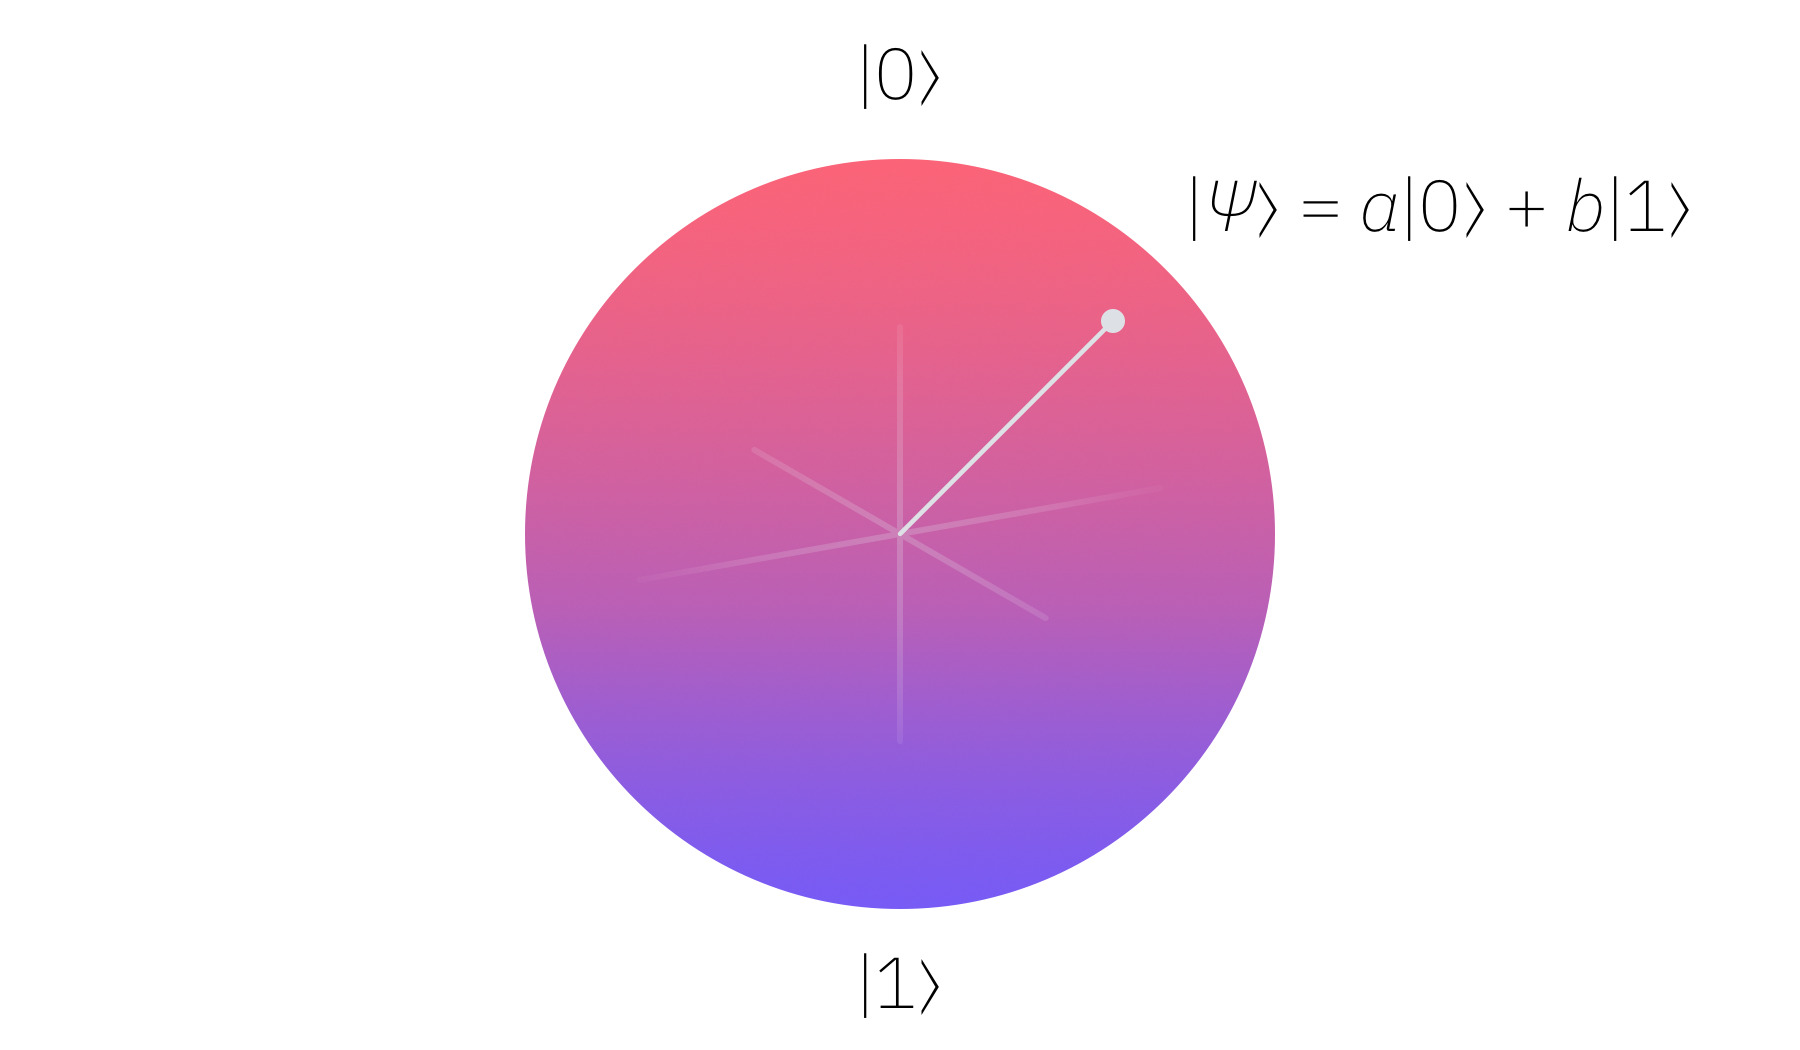
\includegraphics[alt={Testo alternativo dell'immagine}, height=5cm]{img/qubit.jpeg}
    \description[Rappresenzazione Qubit]{Long description}
    \caption{Lorem}
    \label{fig:qubit}
\end{figure}
\lipsum[1]

\section{Processo sviluppo prodotto}
\lipsum[1-2]

\begin{listing}[H]
\begin{minted}{c}
#include <stdio.h>
int main() {
    print("Hello, world!");
    return 0;
}
\end{minted}
\caption{Example of code}
\label{listing:b}
\end{listing}

Lorem ipsum:
\begin{listing}[H]
\begin{minted}{c}
#include <stdio.h>
int main() {
    print("Hello, world!");
    return 0;
}
\end{minted}
\caption{Example of code}
\label{listing:b-2}
\end{listing}

Lorem ipsum:
\begin{listing}[H]
\begin{minted}{c}
#include <stdio.h>
int main() {
    print("Hello, world!");
    return 0;
}
\end{minted}
\caption{Example of code}
\label{listing:b-3}
\end{listing}

\newpage
    \chapter{Descrizione dello stage}
\label{chap:descrizione-stage}

\section{Introduzione al progetto}
\begin{figure}[H] 
    \centering 
    
\includegraphics[alt={Testo alternativo dell'immagine}, width=0.5\columnwidth]{img/pk_estate.jpeg}
    \caption{Caption}
    \label{fig:pk_estate}
\end{figure}
\lipsum[1]

\section{Analisi preventiva dei rischi}

Durante la fase di analisi iniziale sono stati individuati alcuni possibili rischi a cui si potrà andare incontro.
Si è quindi proceduto a elaborare delle possibili soluzioni per far fronte a tali rischi.

\begin{risk}{Performance del simulatore hardware}
    \riskdescription{le performance del simulatore hardware e la comunicazione con questo potrebbero risultare lenti o non abbastanza buoni da causare il fallimento dei test}
    \risksolution{coinvolgimento del responsabile a capo del progetto relativo il simulatore hardware}
    \label{risk:hardware-simulator} 
\end{risk}

\section{Requisiti e obiettivi}

\begin{center}
    \rowcolors{1}{}{tableGray}
    \begin{longtable}{|p{2.25cm}|p{7.75cm}|p{2.25cm}|}
    \hline
    \multicolumn{1}{|c|}{\textbf{A}} & \multicolumn{1}{c|}{\textbf{B}}\\ 
    \hline 
    \endfirsthead
    \rowcolor{white}
    \multicolumn{3}{c}{{\bfseries \tablename\ \thetable{} -- Continuo della tabella}}\\
    \hline
    \multicolumn{1}{|c|}{\textbf{A}} & \multicolumn{1}{c|}{B}\\ \hline 
    \endhead
    \hline
    \rowcolor{white}
    \multicolumn{3}{|r|}{{Continua nella prossima pagina...}}\\
    \hline
    \endfoot
    \endlastfoot 
    
    AA & BB \\
    \hline
    AA & BB \\
    \hline
    AA & BB \\
    \hline
    AA & BB \\
    \hline
    \hiderowcolors
    \caption{Lorem.}
    \label{tab:requisiti_obbiettivi}
    \end{longtable}
\end{center}

\section{Pianificazione}
\begin{figure}[H]
    \centering
    
\includegraphics[alt={Testo alternativo dell'immagine}, width=0.5\columnwidth]{img/pk_estate.jpeg}
    \caption{Caption}
    \label{fig:pk_estate_2}
\end{figure}
\lipsum[1]

\subsection{subsection}
\lipsum[1]

\subsubsection{subsubsection}
\lipsum[1]

\paragraph{paragraph}
\lipsum[1]

\newpage
    \chapter{Analisi dei requisiti}
\label{chap:analisi-requisiti}

\section{Casi d'uso}
Per lo studio dei casi di utilizzo del prodotto sono stati creati dei diagrammi.
I diagrammi dei casi d'uso (in inglese \textit{Use Case Diagram}) sono diagrammi di tipo %\gls{uml}
dedicati alla descrizione delle funzioni o servizi offerti da un sistema, così come sono percepiti e utilizzati dagli attori che interagiscono col sistema stesso.
Essendo il progetto finalizzato alla creazione di un tool %\gls{TermineSenzaAcronimo}
per l'automazione di un processo, le interazioni da parte dell'utilizzatore devono essere ovviamente ridotte allo stretto necessario. Per questo motivo i diagrammi d'uso risultano semplici e in numero ridotto.

\begin{figure}[H]
    \vspace{2em}
    \centering
    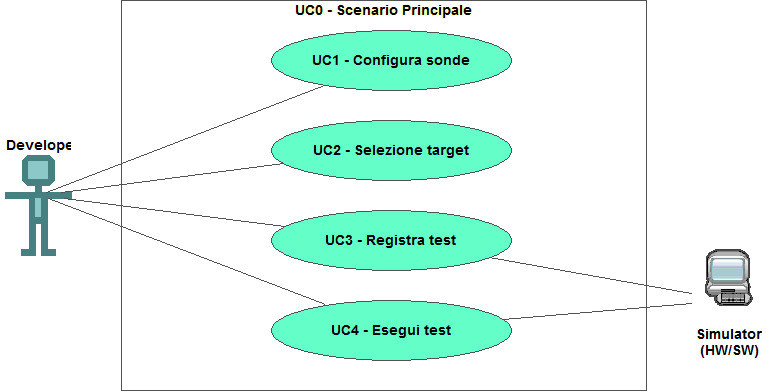
\includegraphics[alt={Testo alternativo dell'immagine}, width=0.75\columnwidth]{img/usecase/scenario-principale.jpeg}
    \caption{Use Case 0: Scenario principale}
    \label{fig:scenario_principale}
\end{figure}

\begin{usecase}{0}{Scenario principale}
    \usecaseactors{Sviluppatore applicativi.}
    \usecasepre{Lo sviluppatore è entrato nel plugin di simulazione all'interno dell'IDE.}
    \usecasedesc{La finestra di simulazione mette a disposizione i comandi per configurare, registrare o eseguire un test.}
    \usecasepost{Il sistema è pronto per permettere una nuova interazione.}
    \label{uc:uc_scenario_principale}
\end{usecase}

\begin{usecase}{1}{Gestione Utente}
    \usecaseactors{Amministratore, Utente Registrato.}
    \usecasepre{L'utente deve essere autenticato nel sistema.}
    \usecasedesc{L'utente può gestire le informazioni del proprio profilo.}
    \usecasepost{Le modifiche vengono salvate nel sistema.}
    \usecasealt{Se l'utente non è autenticato, visualizza un messaggio di errore.}
    \label{uc:uc_casi_uso}
\end{usecase}

\begin{usecase}{2}{Creazione Prodotto}
    \usecaseactors{Amministratore.}
    \usecasepre{L'amministratore ha effettuato l'accesso al sistema.}
    \usecasedesc{L'amministratore può aggiungere un nuovo prodotto al catalogo.}
    \usecasepost{Il nuovo prodotto viene aggiunto con successo.}
    \usecasealt{Se i campi obbligatori non sono compilati, visualizza un messaggio di errore.}
    \label{uc:uc_creazione_prodotto}
\end{usecase}

\section{Tracciamento dei requisiti}
Da un'attenta analisi dei requisiti e degli use case effettuata sul progetto è stata stilata la tabella che traccia i requisiti in rapporto agli use case.\\
Sono stati individuati diversi tipi di requisiti e si è quindi fatto utilizzo di un codice identificativo per distinguerli.\\
Il codice dei requisiti, dove ogni requisito è identificato con il carattere \textbf{R}, è così strutturato:
\begin{enumerate}
    \item[\textbf{F}:] Funzionale.
    \item[\textbf{Q}:] Qualitativo.
    \item[\textbf{V}:] Di vincolo.
    \item[\textbf{N}:] Obbligatorio (necessario).
    \item[\textbf{D}:] Desiderabile.
    \item[\textbf{Z}:] Opzionale.
\end{enumerate}

Nelle tabelle \ref{tab:requisiti_funzionali}, \ref{tab:requisiti_qualitativi} e \ref{tab:requisiti_vincolo} sono riassunti i requisiti e il loro tracciamento con gli use case delineati in fase di analisi.

\section{Tabelle dei requisiti}
\begin{center}
    \rowcolors{1}{}{tableGray}
    \begin{longtable}{|p{2.25cm}|p{7.75cm}|p{2.25cm}|}
    \hline
    %\rowcolor{hyperColor!5}
    \multicolumn{1}{|c|}{\textbf{Requisito}} & \multicolumn{1}{c|}{\textbf{Descrizione}} & \multicolumn{1}{c|}{\textbf{Use Case}}\\
    \hline 
    \endfirsthead
    \rowcolor{white}
    \multicolumn{3}{c}{{\bfseries \tablename\ \thetable{} -- Continuo della tabella}}\\
    \hline
    %\rowcolor{hyperColor!5}
    \multicolumn{1}{|c|}{\textbf{Requisito}} & \multicolumn{1}{c|}{\textbf{Descrizione}} & \multicolumn{1}{c|}{\textbf{Use Case}}\\
    \hline 
    \endhead
    \hline
    \rowcolor{white}
    \multicolumn{3}{|r|}{{Continua nella prossima pagina...}}\\
    \hline
    \endfoot
    \endlastfoot
    
    RFN-1 & L’interfaccia permette di configurare il tipo di sonde del test & UC1 \\
    \hline
    \hiderowcolors
    \caption{Tabella del tracciamento dei requisiti funzionali.}
    \label{tab:requisiti_funzionali}
    \end{longtable}
\end{center}

\begin{center}
    \rowcolors{1}{}{tableGray}
    \begin{longtable}{|p{2.25cm}|p{7.75cm}|p{2.25cm}|}
    \hline
    %\rowcolor{hyperColor!5}
    \multicolumn{1}{|c|}{\textbf{Requisito}} & \multicolumn{1}{c|}{\textbf{Descrizione}} & \multicolumn{1}{c|}{\textbf{Use Case}}\\
    \hline 
    \endfirsthead
    \rowcolor{white}
    \multicolumn{3}{c}{{\bfseries \tablename\ \thetable{} -- Continuo della tabella}}\\
    \hline
    %\rowcolor{hyperColor!5}
    \multicolumn{1}{|c|}{\textbf{Requisito}} & \multicolumn{1}{c|}{\textbf{Descrizione}} & \multicolumn{1}{c|}{\textbf{Use Case}}\\
    \hline 
    \endhead
    \hline
    \rowcolor{white}
    \multicolumn{3}{|r|}{{Continua nella prossima pagina...}}\\
    \hline
    %\caption{Tabella del tracciamento dei requisiti qualitativi.}
    \endfoot
    \endlastfoot
    
    RQD-1n & Le prestazioni del simulatore hardware deve garantire la giusta esecuzione dei test e non la generazione di falsi negativi & - \\
    \hline
    RQD-1n & Le prestazioni del simulatore hardware deve garantire la giusta esecuzione dei test e non la generazione di falsi negativi & - \\
    \hline
    RQD-1n & Le prestazioni del simulatore hardware deve garantire la giusta esecuzione dei test e non la generazione di falsi negativi & - \\
    \hline
    RQD-1n & Le prestazioni del simulatore hardware deve garantire la giusta esecuzione dei test e non la generazione di falsi negativi & - \\
    \hline
    RQD-1n & Le prestazioni del simulatore hardware deve garantire la giusta esecuzione dei test e non la generazione di falsi negativi & - \\
    \hline
    RQD-1n & Le prestazioni del simulatore hardware deve garantire la giusta esecuzione dei test e non la generazione di falsi negativi & - \\
    \hline
    \hiderowcolors
    \caption{Tabella del tracciamento dei requisiti qualitativi.}
    \label{tab:requisiti_qualitativi}
    \end{longtable}
\end{center}

\begin{center}
    \rowcolors{1}{}{tableGray}
    \begin{longtable}{|p{2.25cm}|p{7.75cm}|p{2.25cm}|}
    \hline
    %\rowcolor{hyperColor!5}
    \multicolumn{1}{|c|}{\textbf{Requisito}} & \multicolumn{1}{c|}{\textbf{Descrizione}} & \multicolumn{1}{c|}{\textbf{Use Case}}\\
    \hline 
    \endfirsthead
    \rowcolor{white}
    \multicolumn{3}{c}{{\bfseries \tablename\ \thetable{} -- Continuo della tabella}}\\
    \hline
    %\rowcolor{hyperColor!5}
    \multicolumn{1}{|c|}{\textbf{Requisito}} & \multicolumn{1}{c|}{\textbf{Descrizione}} & \multicolumn{1}{c|}{\textbf{Use Case}}\\
    \hline 
    \endhead
    \hline
    \rowcolor{white}
    \multicolumn{3}{|r|}{{Continua nella prossima pagina...}}\\
    \hline
    \endfoot
    \endlastfoot
    
    RVO-1 & La libreria per l'esecuzione dei test automatici deve essere riutilizzabile & - \\
    \hline
    \hiderowcolors
    \caption{Tabella del tracciamento dei requisiti di vincolo.}
    \label{tab:requisiti_vincolo}
    \end{longtable}
\end{center}

\newpage
    \chapter{Progettazione e codifica}
\label{chap:progettazione-codifica}
Breve introduzione al capitolo

\section{Tecnologie e strumenti}
\label{sec:tecnologie-strumenti}
Di seguito viene data una panoramica delle tecnologie e strumenti utilizzati.

\subsection*{Tecnologia 1}
Descrizione Tecnologia 1.

\subsection*{Tecnologia 2}
Descrizione Tecnologia 2

\section{Ciclo di vita del software}
\label{sec:ciclo-vita-software}

\section{Progettazione}
\label{sec:progettazione}

\subsection{Namespace 1}
Descrizione namespace 1.

\section{Design Pattern utilizzati}

\section{Codifica}
Blocco di codice in C
\begin{listing}[H]
\begin{minted}{c}
#include <stdio.h>
int main() {
    print("Hello, world!");
    return 0;
}
\end{minted}
\caption{Example of code}
\label{listing:c}
\end{listing}

\newpage
    \chapter{Verifica e validazione}
\label{chap:verifica-validazione}

\begin{figure}[H]
    \centering
    
\includegraphics[alt={Testo alternativo dell'immagine}, width=1\columnwidth]{img/quantum_superposition.jpeg}
    \caption{Lorem}
    \label{fig:enter-label}
\end{figure}

\lipsum[1-2]

% Esempio di come importare un file contenente codice
Lorem ipsum:
\begin{listing}[H]
\inputminted{python}{code/example.py}
\caption{Fibonacci recursive}
\label{listing:py_fibo}
\end{listing}

\lipsum[1]

\newpage
    \chapter{Conclusioni}
\label{chap:conclusioni}

\section{Consuntivo finale}


\section{Raggiungimento degli obiettivi}


\section{Conoscenze acquisite}


\section{Valutazione personale}


\section{Valutazione personale}


\newpage

    \pagenumbering{roman}
    \backmatter
    \chapter{Bibliografia}
\label{cap:bibliography}

\nocite{*}

% Books bibliography
\printbibliography[heading=subbibliography, title={Testi}, type=book]

% Articles bibliography
\printbibliography[heading=subbibliography, title={Articoli}, type=article]

% Websites bibliography
%\printbibliography[heading=subbibliography, title={Siti}, type=online]

    \chapter{Sitografia}
\label{cap:webliography}
\nocite{*}

% Websites bibliography
\printbibliography[heading=subbibliography, title={\null}, type=online]

\end{document}